$\lambda=$
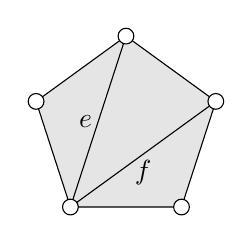
\begin{tikzpicture}[every node/.style={inner sep=2pt},baseline=(ref.base)]
\foreach \t in {1,...,5}
\coordinate (v\t) at ({18+72*\t}:1.2);
\draw[fill=gray!20] (v1) -- (v2) -- (v3) -- (v4) -- (v5) -- cycle;
\draw (v1) -- node[left]{$e$} (v3) -- node[below]{$f$} (v5);
\foreach \t in {1,...,5}
\draw[fill=white] (v\t)circle(0.1);
\node (ref) at (0,0) {\phantom{$-$}};
\end{tikzpicture}
$\longrightarrow$
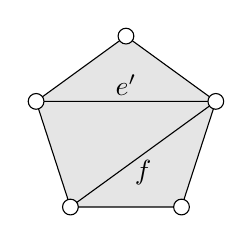
\begin{tikzpicture}[every node/.style={inner sep=2pt},baseline=(ref.base)]
\foreach \t in {1,...,5}
\coordinate (v\t) at ({18+72*\t}:1.2);
\draw[fill=gray!20] (v1) -- (v2) -- (v3) -- (v4) -- (v5) -- cycle;
\draw (v2) -- node[above]{$e'$} (v5) -- node[below]{$f$} (v3);
\foreach \t in {1,...,5}
\draw[fill=white] (v\t)circle(0.1);
\node (ref) at (0,0) {\phantom{$-$}};
\end{tikzpicture}
$\longrightarrow$
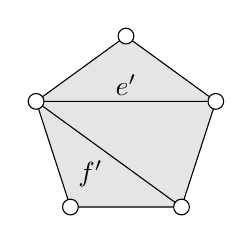
\begin{tikzpicture}[every node/.style={inner sep=2pt},baseline=(ref.base)]
\foreach \t in {1,...,5}
\coordinate (v\t) at ({18+72*\t}:1.2);
\draw[fill=gray!20] (v1) -- (v2) -- (v3) -- (v4) -- (v5) -- cycle;
\draw (v5) -- node[above]{$e'$} (v2) -- node[below left]{$f'$} (v4);
\foreach \t in {1,...,5}
\draw[fill=white] (v\t)circle(0.1);
\node (ref) at (0,0) {\phantom{$-$}};
\end{tikzpicture}

$\longrightarrow$
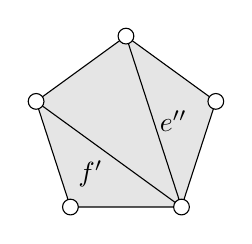
\begin{tikzpicture}[every node/.style={inner sep=2pt},baseline=(ref.base)]
\foreach \t in {1,...,5}
\coordinate (v\t) at ({18+72*\t}:1.2);
\draw[fill=gray!20] (v1) -- (v2) -- (v3) -- (v4) -- (v5) -- cycle;
\draw (v1) -- node[right]{$e''$} (v4) -- node[below left]{$f'$} (v2);
\foreach \t in {1,...,5}
\draw[fill=white] (v\t)circle(0.1);
\node (ref) at (0,0) {\phantom{$-$}};
\end{tikzpicture}
$\longrightarrow$
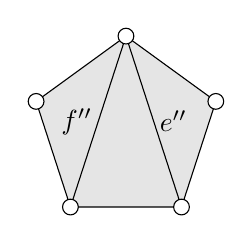
\begin{tikzpicture}[every node/.style={inner sep=2pt},baseline=(ref.base)]
\foreach \t in {1,...,5}
\coordinate (v\t) at ({18+72*\t}:1.2);
\draw[fill=gray!20] (v1) -- (v2) -- (v3) -- (v4) -- (v5) -- cycle;
\draw (v4) -- node[right]{$e''$} (v1) -- node[left]{$f''$} (v3);
\foreach \t in {1,...,5}
\draw[fill=white] (v\t)circle(0.1);
\node (ref) at (0,0) {\phantom{$-$}};
\end{tikzpicture}
$\longrightarrow$
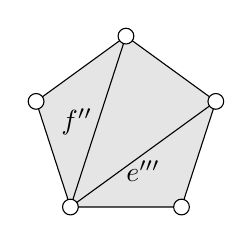
\begin{tikzpicture}[every node/.style={inner sep=2pt},baseline=(ref.base)]
\foreach \t in {1,...,5}
\coordinate (v\t) at ({18+72*\t}:1.2);
\draw[fill=gray!20] (v1) -- (v2) -- (v3) -- (v4) -- (v5) -- cycle;
\draw (v5) -- node[below]{$e'''$} (v3) -- node[left]{$f''$} (v1);
\foreach \t in {1,...,5}
\draw[fill=white] (v\t)circle(0.1);
\node (ref) at (0,0) {\phantom{$-$}};
\end{tikzpicture}
$=\lambda$.